%%%%%%%%%%%%%%%%%%%%%%%%%%%%%%%%%%%%%%%%%
% baposter Landscape Poster
% LaTeX Template
% Version 1.0 (11/06/13)
%
% baposter Class Created by:
% Brian Amberg (baposter@brian-amberg.de)
%
% This template has been downloaded from:
% http://www.LaTeXTemplates.com
%
% License:
% CC BY-NC-SA 3.0 (http://creativecommons.org/licenses/by-nc-sa/3.0/)
%
%%%%%%%%%%%%%%%%%%%%%%%%%%%%%%%%%%%%%%%%%

%----------------------------------------------------------------------------------------
%	PACKAGES AND OTHER DOCUMENT CONFIGURATIONS
%----------------------------------------------------------------------------------------

\documentclass[landscape,a0paper,fontscale=0.285]{baposter} % Adjust the font scale/size here

\usepackage{graphicx} % Required for including images
\graphicspath{{figures/}} % Directory in which figures are stored

\usepackage{amsmath} % For typesetting math
\usepackage{amssymb} % Adds new symbols to be used in math mode

\usepackage{booktabs} % Top and bottom rules for tables
\usepackage{enumitem} % Used to reduce itemize/enumerate spacing
\usepackage{palatino} % Use the Palatino font
\usepackage[font=small,labelfont=bf]{caption} % Required for specifying captions to tables and figures

\usepackage{multicol} % Required for multiple columns
\setlength{\columnsep}{1.5em} % Slightly increase the space between columns
\setlength{\columnseprule}{0mm} % No horizontal rule between columns

\usepackage{tikz} % Required for flow chart
\usetikzlibrary{shapes,arrows} % Tikz libraries required for the flow chart in the template

\newcommand{\compresslist}{ % Define a command to reduce spacing within itemize/enumerate environments, this is used right after \begin{itemize} or \begin{enumerate}
\setlength{\itemsep}{1pt}
\setlength{\parskip}{0pt}
\setlength{\parsep}{0pt}
}

\definecolor{lightblue}{rgb}{0.145,0.6666,1} % Defines the color used for content box headers

\begin{document}

\begin{poster}
{
headerborder=closed, % Adds a border around the header of content boxes
colspacing=1em, % Column spacing
bgColorOne=white, % Background color for the gradient on the left side of the poster
bgColorTwo=white, % Background color for the gradient on the right side of the poster
borderColor=lightblue, % Border color
headerColorOne=black, % Background color for the header in the content boxes (left side)
headerColorTwo=lightblue, % Background color for the header in the content boxes (right side)
headerFontColor=white, % Text color for the header text in the content boxes
boxColorOne=white, % Background color of the content boxes
textborder=roundedleft, % Format of the border around content boxes, can be: none, bars, coils, triangles, rectangle, rounded, roundedsmall, roundedright or faded
eyecatcher=true, % Set to false for ignoring the left logo in the title and move the title left
headerheight=0.1\textheight, % Height of the header
headershape=roundedright, % Specify the rounded corner in the content box headers, can be: rectangle, small-rounded, roundedright, roundedleft or rounded
headerfont=\Large\bf\textsc, % Large, bold and sans serif font in the headers of content boxes
%textfont={\setlength{\parindent}{1.5em}}, % Uncomment for paragraph indentation
linewidth=2pt % Width of the border lines around content boxes
}
%----------------------------------------------------------------------------------------
%	TITLE SECTION 
%----------------------------------------------------------------------------------------
%
{
\includegraphics[height=4em]{loopq.png}}
{\bf\textsc{Loop Q PRIZE Qualifying Challenge 2019}\vspace{0.1em}} % Poster title
{\textsc{\{ Michal Ostyk-Narbutt \} \hspace{10pt} Sapienza University of Rome}} % Author names and institution
{
\includegraphics[height=4em]{loopq.png}} % Second university/lab logo on the right

%----------------------------------------------------------------------------------------
%	INTRODUCTION
%----------------------------------------------------------------------------------------

\headerbox{Introduction}{name=conclusion,column=0,span=1,row=0}{
The Willy Wonka chocolate factory produces the \textbf{Golden Scrumpilicious Candy Bar}, which packaged in a golden wrapper. However, sometimes during production the bars end up being green which is a defect, but also very alluring and well selling.\\ Given data from the production line from 60 Oompa-Loompa's, the goal is to predict the production of the \textbf{green bars}. \\
In this presentation I will go over the overview of the solution, its design criteria, and its strengths. 

}

%----------------------------------------------------------------------------------------
%	OBJECTIVES
%----------------------------------------------------------------------------------------

\headerbox{Methodology}{name=methodology, column=1,span=1,row=0}{
The training pipeline(right), depicts the approach to the solution.  At first, an SVM model was applied to the imbalanced data, but seeing that data is hard to marginalise in Figure \ref{pca}, it gave really poor results. Hence,  Random forests (RF) were used since model architecture reduces overfitting  However, to improve results oversampling using SMOTE was peformed. RF precision and recall gave better results on a balanaced dataset. Note that in cross-validation (CV) with oversampling, only the training fold was oversampled.



%\vspace{0.3em} % When there are two boxes, some whitespace may need to be added if the one on the right has more content
}



%----------------------------------------------------------------------------------------
%	DATASET
%----------------------------------------------------------------------------------------

\headerbox{Dataset}{name=dataset,column=0,span=2,row=1, below=methodology}{


%------------------------------------------------

\begin{multicols}{2}
\begin{center}
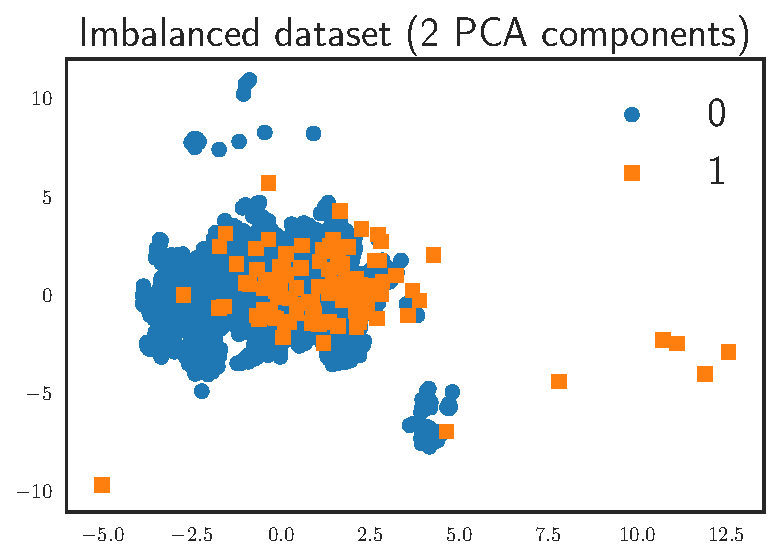
\includegraphics[width=0.8\linewidth]{Imbalanced_dataset_(2_PCA_components)pca.pdf}
\captionof{figure}{Normalised data with applied PCA dimensionality reduction. The plot shows how extreamly difficult it is to distinguish between golden and green bars.}
\label{pca}
\end{center}

%\begin{center}
%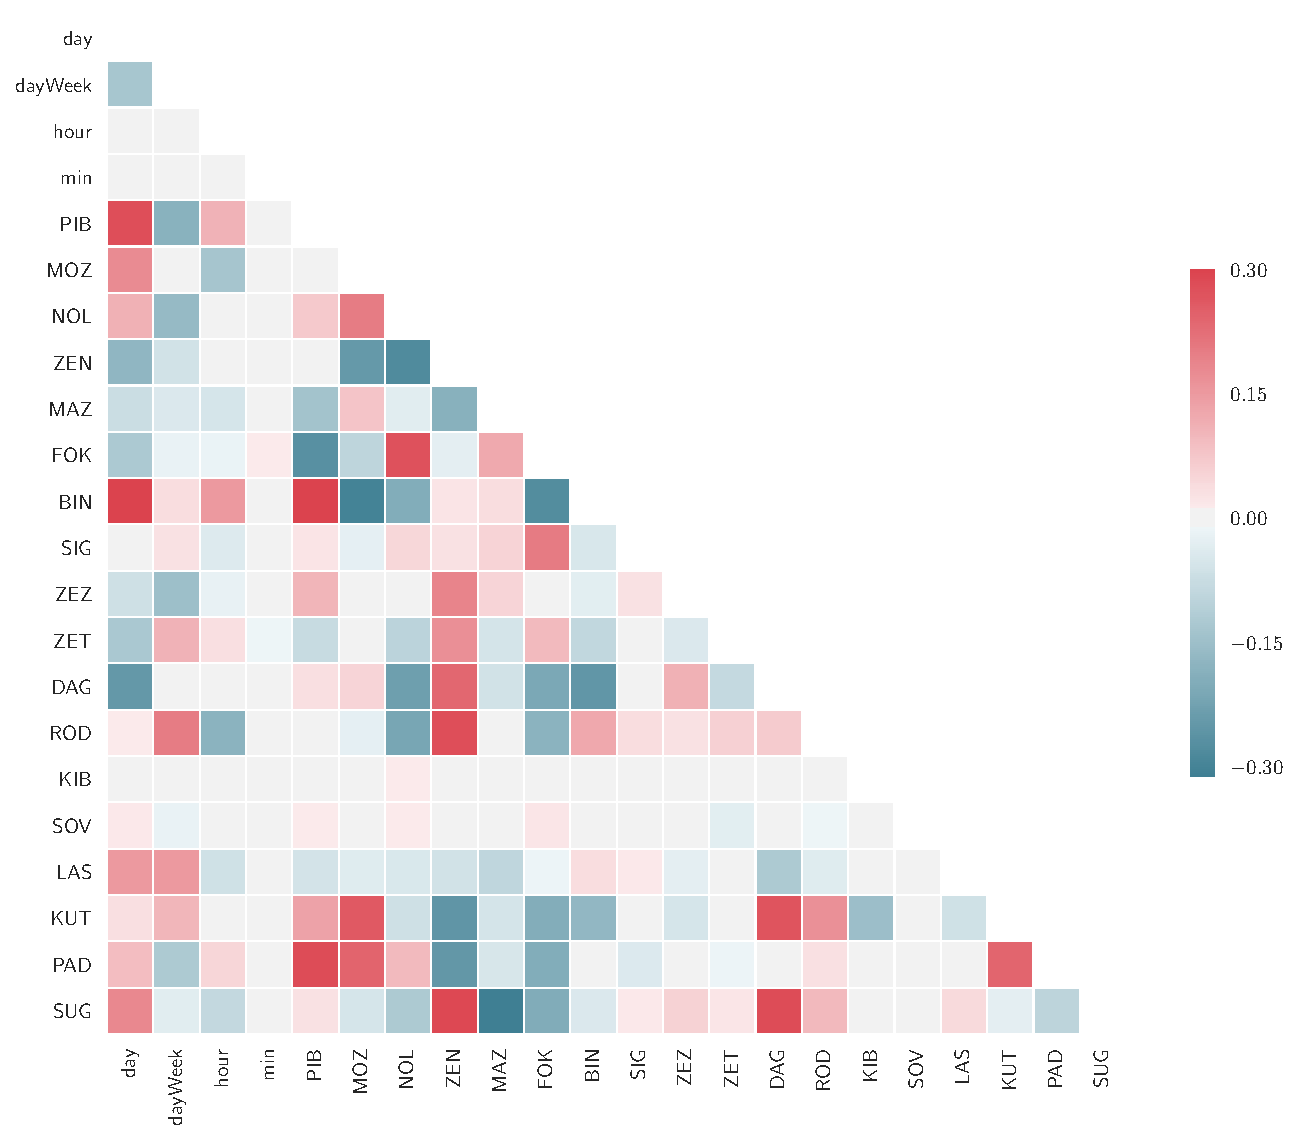
\includegraphics[width=0.8\linewidth]{correlation.pdf}
%\captionof{figure}{Correlation matrix after removing correlated features with lower and upper bound threshold equal to -0.31, and 0.31 respectively}
%\end{center}
%------------------------------------------------
The dataset given consits of 62 columns, of which 60 are scalar features given by each Oompa-Loompa, 1 is a time stamp, and the last is the target 'GREEN'. This task will consist of binary classification. However, the data is immensely imbalanced as green bar production is very rare.
\begin{center}
\begin{tabular}{l l}
\toprule
\textbf{Golden bars} & \textbf{Green bars} \\
\midrule
15704 & 102 \\
\bottomrule
\end{tabular}
\captionof{table}{Gold vs Green bars in dataset}
\end{center}
Feature engineering involved of decomposing the time stamp into 5 columns : "day", "dayWeek", "hour", "min", "month". Moreover, Features correlated with each other by a threshold $t=\pm 0.32$  were discarded. Hence, the training  and testing was done on 22 features.
\end{multicols}


%\vspace{1em}
\begin{center}
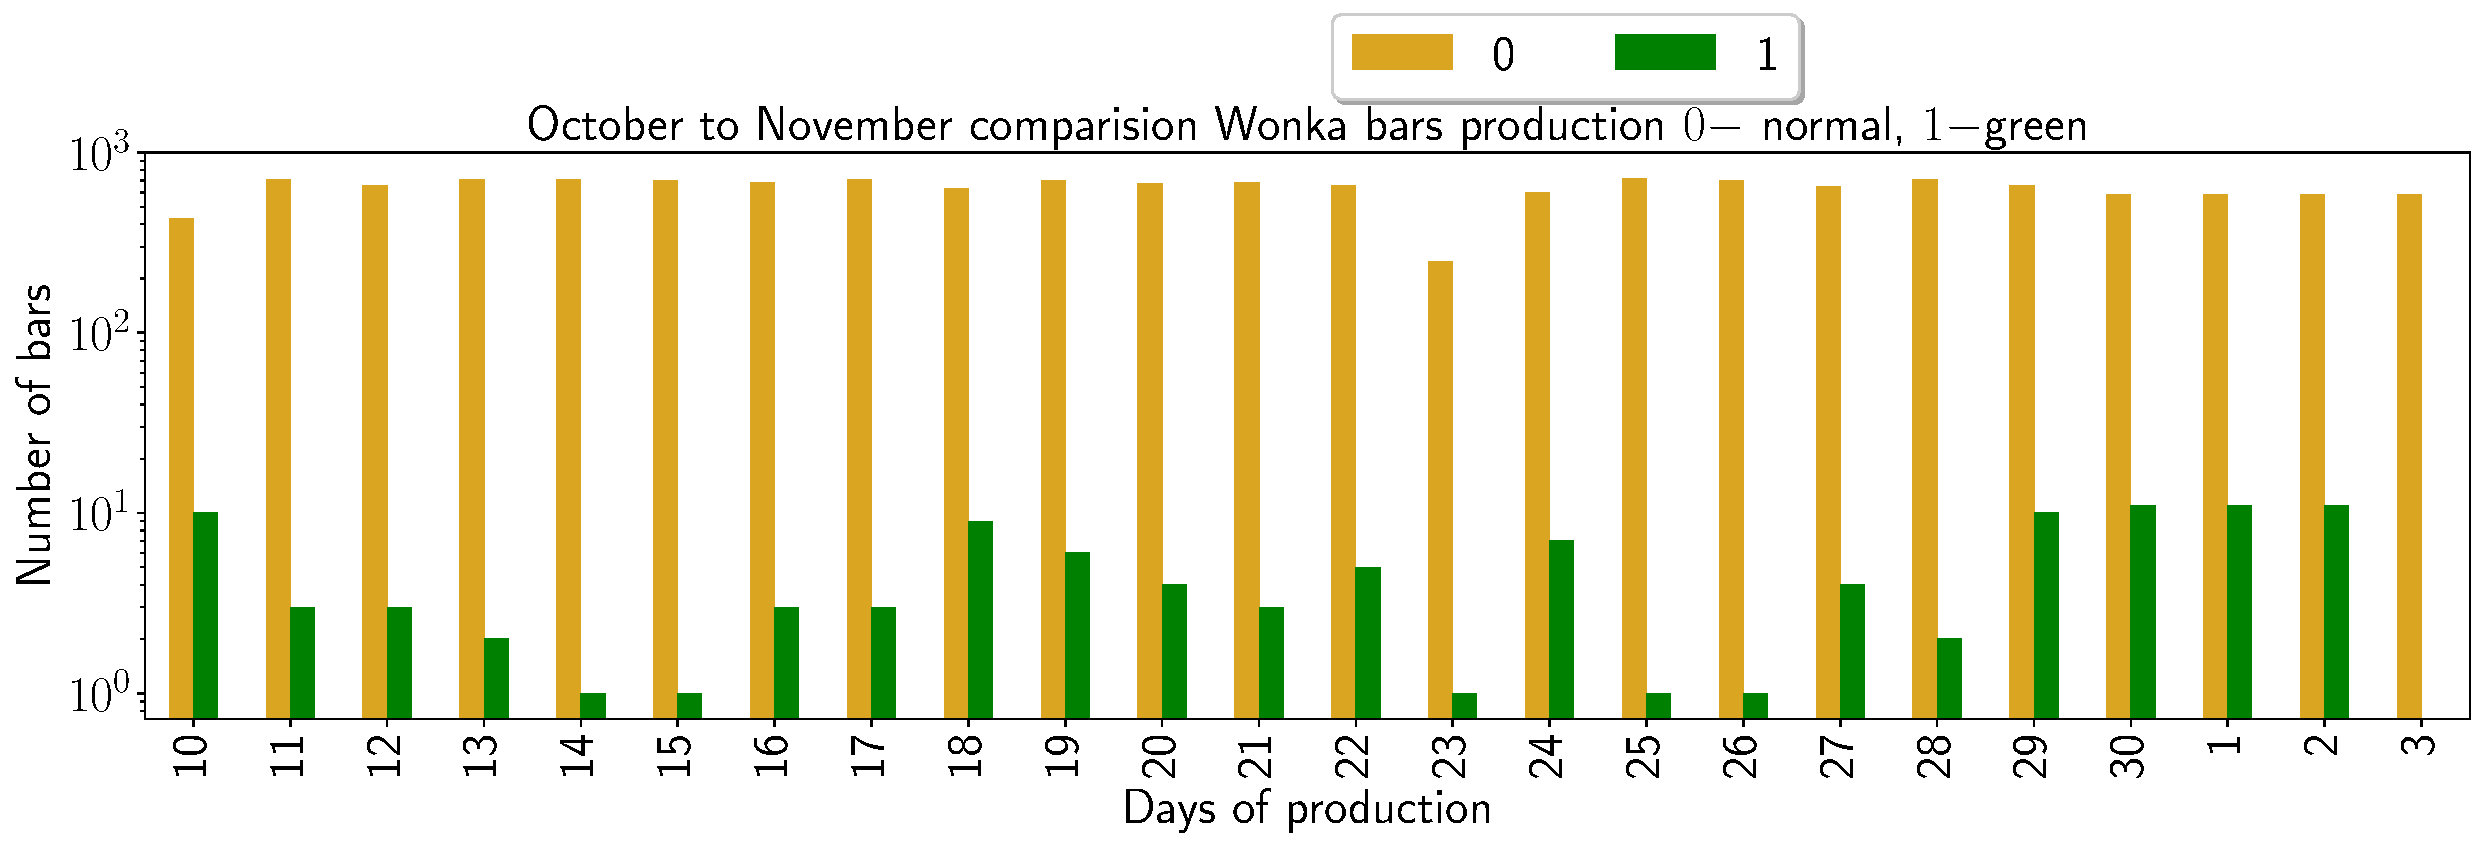
\includegraphics[width=\linewidth]{data_overview.pdf}
\captionof{figure}{Analysis of production of gold(0) and green(1) chocolate bars through October to early November 2018}
\end{center}
}


%----------------------------------------------------------------------------------------
%	MATERIALS AND METHODS
%----------------------------------------------------------------------------------------

\headerbox{Training Pipeline}{name=training, row= 0, column=2, span = 2}{ % This block's bottom aligns with the bottom of the conclusion block
\tikzstyle{decision} = [diamond, draw, fill=blue!20, text width=4.5em, text badly centered, node distance=3cm, inner sep=0pt]
\tikzstyle{block} = [rectangle, draw, fill=blue!20, text width=7em, text centered, rounded corners, node distance=3cm, minimum height=4em]
\tikzstyle{line} = [draw, -latex' ]
\tikzstyle{cloud} = [draw, ellipse, fill=red!20, node distance=3cm, minimum height=2em]
\tikzstyle{block2} = [rectangle, draw, fill=blue!20, text width=8em, text centered, rounded corners, node distance=3cm, minimum height=6em]

\begin{tikzpicture}[node distance = 2cm, auto]
\node [block] (init) {Feature engineering \& correlation check};
\node [cloud, left of=init] (train) {Training data};
\node [block, below of=init] (drop) {feature drop};
\node [cloud, right of=init] (test) {Test data};
\node [block, below of=drop] (CV) {Cross-validation gridsearch};

\node [block, left of=drop] (imbData) {Imbalanced data};
\node [block, right of=CV] (balData) {Balanced data (via Oversampling)};
\path [line] (CV) -- (balData);
\path [line] (CV) -- (imbData);

\node [decision, below of=imbData] (svm) {Random Forest $-$ poor results };
\node [block, right of=balData] (rf) {Random Forest(RF) $-$ better results};
\path [line] (imbData) -- (svm);
\path [line] (balData) -- (rf);

\node [block, right of=rf] (rff) {RF using best hyperparameters};
\path [line] (rf) -- (rff);
\node [block2, above of=rff] (model) {split into oversampling(train), val, test};
\path [line] (rff) -- (model);

\node [block, left of=model] (trainmodel) {Train model and save};
\path [line] (model) -- (trainmodel);

\node [block, above of=trainmodel] (finalmodel) {Final model};
\path [line] (trainmodel) -- (finalmodel);

\path [line] (test) -- (finalmodel);

\node [decision, right of=finalmodel] (preds) {predictions in CSV};
\path [line] (finalmodel) -- (preds);

\path [line] (init) -- (drop);
\path [line] (drop) -- (CV);
\path [line, dashed] (train) -- (init);
\path [line, dashed] (test) -- (drop);
\path [line, dashed] (drop) -| (test);
\end{tikzpicture}
}


%----------------------------------------------------------------------------------------
%	Results
%----------------------------------------------------------------------------------------

\headerbox{Results}{name=results,column=2, span=2, below=training}{ % This block's bottom aligns with the bottom of the conclusion block
The training consisted of a grid-search K-fold cross validation to find the best hyperparameters (Best-hp). Seeing that balanced data gave better results (Table 2), and using their Best-hp, training was performed on the entire dataset split into: train, validation, and test. Only train was oversampled.

\begin{center}
\begin{tabular}{l l l l l}
\toprule
\textbf{Model Type} & \textbf{Accuracy} & \textbf{Precision} & \textbf{Recall} & \textbf{F1-score}\\
\midrule
CV Imblanced RF & 0.9960$\pm$0.0006 & 0.91$\pm$0.05 & 0.41$\pm$0.08 & 0.9952$\pm$0.0008\\
CV Balanced RF  &  0.9947$\pm$0.0011 & 0.67$\pm$0.18 & 0.402$\pm$0.017 & 0.9941$\pm$0.0009\\
Best-hp $validation$ macro average & 0.99 & 1    & 0.75    &   0.83\\
Best-hp $test$ macro average & 0.99 & 0.96  &    0.68      &0.76\\
\bottomrule
\end{tabular}
\label{res}
\captionof{table}{End results of training on balanced and imbalanced datasets $+$ final training on the best hyperparamters.}
\end{center}
}
%----------------------------------------------------------------------------------------

%----------------------------------------------------------------------------------------
%	CONCLUSIONS
%----------------------------------------------------------------------------------------

\headerbox{Conclusions}{name=conclusions,column=2, span=2, below=results}{ % This block's bottom aligns with the bottom of the conclusion block
Random forests are great estimators when their is a significant amount of collinerity on an imbalanced dataset. However, reducing that collinerity and oversampling the training set, results in better overall performance. In this task however, we are largly concered with recall than precision. This is because, it is far more costly to wrongly predict a green bar as gold, rather than vice-versa and hence letting a green bar simply slip by. The percentage of green bars in the training dataset is $0.65 \%$ meanwhile, the percentage on the given test dataset predicted by the best model is just over 1 percent. Hence to conclude, I reckon that the model should yield good results once tested by the judges, as greens are rare as potrayed in Figure 2.\\
Please note: logos in the top left and right belong to and were taken from <www.loopqprize.ai>
}
%---



%
%%----------------------------------------------------------------------------------------
%%	REFERENCES
%%----------------------------------------------------------------------------------------
%
%\headerbox{References}{name=references,column=3,above=bottom}{
%
%\renewcommand{\section}[2]{\vskip 0.05em} % Get rid of the default "References" section title
%\nocite{*} % Insert publications even if they are not cited in the poster
%\small{ % Reduce the font size in this block
%\bibliographystyle{unsrt}
%\bibliography{sample} % Use sample.bib as the bibliography file
%}}



\end{poster}

\end{document}